\documentclass{sintefbeamer}

% packages, font, color, and newcommands
\usepackage{amsfonts, amsmath, oldgerm, lmodern, bm}
% \usepackage[font={footnotesize}]{caption}
\usepackage{natbib}
\usepackage{url}
\usepackage{tikz}
\usepackage{amssymb}
\usepackage{amsmath}
\usepackage{amsthm}
\usepackage{mathrsfs}
\usepackage{empheq}
\usepackage{mdframed}
\usepackage{bm}
\usepackage{animate}
\usepackage{xcolor,colortbl}
\usepackage{graphicx}
\usepackage{pgfplots}
\bibliographystyle{apalike}
\usefonttheme{serif}
\usetikzlibrary{calc}

\title{Theoretical prediction of the Reynolds stress in low inertial buoyant emulsion.}
\subtitle{Based on the nearest particle statistic}
\author{\href{http://basilisk.fr/sandbox/fintzin/Rising-Suspenion/RS.c}{\underline{N. Fintzi}\footnote{IFP \'Energies Nouvelles, France}$^{,2}$}, JL. Pierson$^1$ and S. Popinet\footnote{Sorbonne Universit\'e, France}}
% \date{Created on May 22, 2022}

\titlebackground{image/700drop.png}

% document body
\addtobeamertemplate{navigation symbols}{}{%
    \usebeamerfont{footline}%
    \usebeamercolor[fg]{footline}%
    % \hspace{1em}%
    % \vspace{1em}%
    \insertframenumber/\inserttotalframenumber
}
\usepackage{stmaryrd}

\usepackage{amsmath}


\begin{document}
\maketitle


\begin{frame}
  \frametitle{Industrial context}
  \underline{Coalescence is ubiquitous in chemical engineering processes :}
  \begin{itemize}
    \item Separation processes (gravity separators, flotation)
    \item Bubble column reactors
    \item Liquid-liquid separation
  \end{itemize}
  \vfill
  \underline{In all those process we need to : }
  \begin{itemize}
    \item Predict global hydrodynamics in disperse bubbly flows and emulsion with 
    the \textbf{Euler-Euler} two-fluid models. 
    \begin{itemize}
      \item Model for the interphase drag forces.
      \item Model for the \textbf{Reynolds stress}.
      \item Model of coalesce and size distribution 
      % \begin{itemize}
      %   \item Describe the interactions between pairs of droplets
      %   \item Predict interaction frequency
      %   \item Predict film drainage time 
      % \end{itemize}
    \end{itemize}
  \end{itemize}

  \vfill
$\to$ In this presentation we focus on the \textbf{Reynolds Stress} or \textbf{pseudo turbulent} tensor modeling. 
\end{frame}

\section{Introduction : what is the Reynolds stress ?}

\begin{frame}{To model the processes we use Euler-Euler model }
  Averaged \textbf{mass} and \textbf{momentum} equations for the continuous phase :
\begin{align*}
  % \phi_d + \phi_f &= 1\\
  \pddt (\phi_f \rho_f)  
  + \div (\phi_f \rho_f\textbf{u}_f)
  &= 
  0\\
  \pddt (\phi_f \rho_f\textbf{u}_f)  
  + \div (
      \phi_f \rho_f\textbf{u}_f\textbf{u}_f
      + \bm{\sigma}_f^\text{eff}
  )
  &= 
  \phi_f  \rho_f \textbf{g}
  + 
  \underbrace{
    \avg{\delta_I \bm{\sigma}_f^0 \cdot \textbf{n}_f}
  }_\text{Interphase force}
\end{align*}
With the effective stress : 
\begin{align*}
  &\bm{\sigma}_k^\text{eff}
  = 
   \underbrace{\rho_k\avg{\chi_k \textbf{u}_k'\textbf{u}_k'}}_\text{Reynolds stress}
    - \underbrace{\phi_k \bm{\sigma}_k}_\text{Newtonian stress}
\end{align*}
\begin{itemize}
  \item $\textbf{u}_f$ mean velocity of the fluid phase.  
  \item $\rho_f$ : density of the continuous phase. 
  \item $\phi_f$ : volume fraction of the continuous phase. 
  \item $\avg{\ldots}$ : the ensemble average operator. 
  \item $\textbf{u}_f' = \textbf{u}^0_f - \textbf{u}_f$ where $\textbf{u}_f^0$ is the local (non-averaged) fluid velocity. 
\end{itemize}
\end{frame}





\begin{frame}{Objectives and Hypothesis :}
  \begin{itemize}
    \item Objectives :
    Derive an analytical formula for $\avg{\chi_f \textbf{u}_f'\textbf{u}_f'}$. 
    \item Assuming : 
    \begin{itemize}
      \item Negligible inertia (\textbf{Stokes} regime)
      \item Dilute regime such that $\phi^{2} \approx 0$ 
      \item Mono-disperse suspension of droplets of radius $a$
    \end{itemize}
  \end{itemize}

  
  In this specific situation we can write  (Bachelor 1972) :
  \begin{equation*}
    \avg{\chi_k \textbf{u}'_k\textbf{u}'_k}(\textbf{x},t)
    = 
    n_p(\textbf{x},t)
    \int_{|\textbf{r}| > a }
     \textbf{u}^1\textbf{u}^1(\textbf{r}|\textbf{x}) d\textbf{r}
    +\mathcal{O}(\phi^2)
\end{equation*}

\begin{itemize}
  \item $n_p$ is the number density of particles ;
  \item $\textbf{u}^1(\textbf{r}|\textbf{x})$ : disturbance fields of an isolated droplet located at \textbf{x}. 
\end{itemize}
\end{frame}

\begin{frame}
  \frametitle{L.Van Wijngaarden approach for potential flow.}

The potential flow solution of an isolated translating spheres is :
\begin{equation*}
  \textbf{u}'_\text{potential}
  = \frac{a^3 \textbf{U}}{2}\left(\frac{1}{r^3} - \frac{3 \textbf{xx}}{r^5}\right).
  \text{    for    }r>a
\end{equation*}

Therefore, the Reynolds stress approximation in homogeneous dilute suspension of spherical bubbles can be written Wijngaarden(1976): 
  \begin{align*}
    \avg{\chi_k \textbf{u}'_k\textbf{u}'_k}(\textbf{x},t)
    = \phi \left(\frac{3}{20} U^2\textbf{I} + \frac{1}{20}\textbf{UU} \right)
\end{align*}


\begin{itemize}
  \item $\phi$ is the volume fraction of the dispersed phase. 
  \item $\textbf{U} = \textbf{u}_f-\textbf{u}_p$ is the relative velocity between phases. 
  \item The integral converge because $\textbf{u}_\text{potential}  \sim r^{-3}$
\end{itemize}

\underline{$\to$ We aim for the same closure but in Stokes regime}

\end{frame}

\begin{frame}
  \frametitle{Stokes flow around a translating spherical drop}
  The stokes flow solution of an isolated translating drop is :
  \begin{columns}
    \column{0.6\textwidth}
  \begin{multline*}
    \textbf{u}_\text{stokes} 
    = \left(\frac{ \textbf{I}}{r} + \frac{\textbf{rr}}{r^3}\right)  \frac{1}{4}\left(\frac{3\lambda + 2}{\lambda +1}\right) a \textbf{U}\\
    - \left(-\frac{\textbf{I}}{r^3} + \frac{3 \textbf{rr} }{r^5}\right)  \frac{1}{4}\left(\frac{\lambda}{\lambda +1}\right) a^3 \textbf{U}
  \end{multline*}
  \begin{itemize}
      \item $\lambda$ is the viscosity ratio.
  \end{itemize}

  In this case : 
  \begin{align*}
    \avg{\chi_k \textbf{u}'_k\textbf{u}'_k}(\textbf{x},t)
    &\approx n_p(\textbf{x},t)\int_{|\textbf{r}| > a} \textbf{u}'_\text{stokes}\textbf{u}'_\text{stokes}   d\textbf{r}
    % - \phi_k \textbf{u}_k\textbf{u}_k
    =\infty 
  \end{align*}
  \underline{\textbf{The integral diverges}  ! (beacause $\textbf{u}_\text{stokes} \sim r^{-1}$).}


  \column{0.3\textwidth}
  \begin{figure}
    \caption{velocity fields around an isolated translating droplet}
    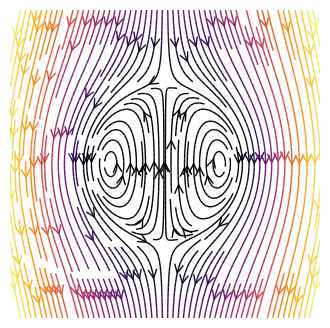
\includegraphics[width=\textwidth]{image/Rising_Stokes.png}
  \end{figure}
  \end{columns}
\end{frame}

\section{The Nearest Particle Statistics}

\begin{frame}{The Nearest Particle Statistics (NPS) approach (DZ Zhang, PoF, 2023)}
  $P_\text{nst}(\textbf{r}|\textbf{x})$ is the probability of finding a nearest particle at \textbf{r} knowing \textbf{x} is occupied by the continuous phase.   

  In the dilute, isotropic and homogeneous regime : 
  \begin{equation}
    P_\text{nst}(r)
    = \frac{3\phi}{4\pi}
    e^{ - \phi (r^3 - 1) }
    \text{ for }
    |\textbf{r}| > a 
  \end{equation}
\begin{columns}
  \column{0.5\textwidth}
  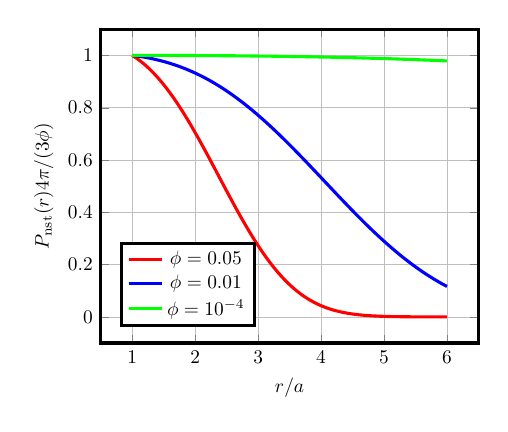
\begin{tikzpicture}[scale=0.7]
    \begin{axis}[
        xlabel={$r/a$},
        ylabel={$P_\text{nst}(r) 4\pi/ (3\phi) $},
        legend style={at={(0.05,0.05)}, anchor=south west},
        grid=major,
        domain=1:6,
        samples=100,
        ultra thick
    ]
    
    % Plot for phi = 0.05
    \addplot[color=red,ultra thick]
    { exp(-0.05 * (x^3 - 1))};
    \addlegendentry{$\phi = 0.05$}
    
    % Plot for phi = 0.01
    \addplot[color=blue,ultra thick]
    { exp(-0.01 * (x^3 - 1))};
    \addlegendentry{$\phi = 0.01$}
    
    % Plot for phi = 0.001
    \addplot[color=green,ultra thick]
    { exp(-0.0001 * (x^3 - 1))};
    \addlegendentry{$\phi = 10^{-4}$}
    
    \end{axis}
\end{tikzpicture}
\column{0.5\textwidth}

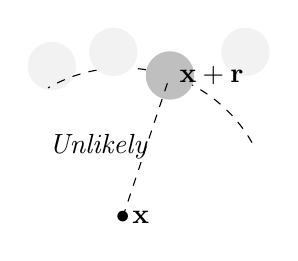
\begin{tikzpicture}[scale=0.6]
  \filldraw[ gray!10!white](+2.6,3.5)circle (0.5);
  \filldraw[ gray!10!white](-1.5,3.2)circle (0.5);
  \draw[dashed](30:3.16) arc (30:120:3.16);
  % \filldraw[ gray!50!white](0,0) circle (0.5);
  \filldraw[ gray!50!white](1,3)circle (0.5);
  \filldraw[ gray!10!white](-0.2,3.5)circle (0.5);
  \draw(0,0)node{$\bullet$}node[right]{$\textbf{x}$};
  \draw[dashed](0,0)--(1,3)node[right]{$\textbf{x}+\textbf{r}$};
  % \draw[dashed](-0.2,3.5);
  \node[ultra thick] (title) at (-0.5,1.5) {\textit{Unlikely}};
\end{tikzpicture} 
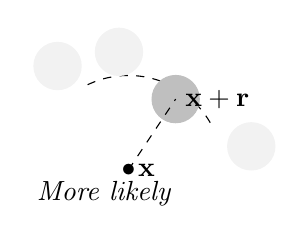
\begin{tikzpicture}[scale=0.6]
  \filldraw[ gray!10!white](+2.6,0.5)circle (0.5);
  \filldraw[ gray!10!white](-1.5,2.2)circle (0.5);
  \draw[dashed](30:2) arc (30:120:2);
  % \filldraw[ gray!50!white](0,0) circle (0.5);
  \filldraw[ gray!50!white](1,1.5)circle (0.5);
  \filldraw[ gray!10!white](-0.2,2.5)circle (0.5);
  \draw(0,0)node{$\bullet$}node[right]{$\textbf{x}$};
  \draw[dashed](0,0)--(1,1.5)node[right]{$\textbf{x}+\textbf{r}$};
  % \draw[dashed](-0.2,3.5);
  \node[ultra thick] (title) at (-0.5,-0.5) {\textit{More likely}};
\end{tikzpicture} 

\end{columns}

\end{frame}


\begin{frame}
  \frametitle{The Reynolds stress decomposition with NPS}
  \begin{equation*}
    \frac{\avg{\chi_f \textbf{u}'_f\textbf{u}'_f}}{\phi_f}(\textbf{x},t)
    = 
    \underbrace{\int 
      \textbf{u}^\text{nst}_f
      \textbf{u}^\text{nst}_f 
      P_\text{nst}(\textbf{r}|\textbf{x}) d\textbf{r} 
    }_\text{Averaged wake contribution}
    + \underbrace{ 
      \int \avg{\delta_i h_i \chi_f \textbf{v}_f''\textbf{v}_f''}  d\textbf{r}
    % P_{nst}(\textbf{x},t,\textbf{r}) d\textbf{r}
    }_{\mathcal{O}(\phi^2)}
  \end{equation*}

\begin{itemize}
  \item $\textbf{u}^\text{nst}(\textbf{x}|\textbf{y})$ Averaged fluctuating value of the fluid phase velocity at \textbf{x}, knowing the nearest particle is located at \textbf{y}
  \item $\textbf{v}''_f = \textbf{u}^0_f - \textbf{u}^\text{nst}_f$ fluctuating values of the local velocity $\textbf{u}_f^0$ (non-averaged) around the conditionally averaged velocity wake at \textbf{x} knowing the nearest neighbor at \textbf{r}.
  \item This relation is exact and require no assumption. 
\end{itemize}
\end{frame}


\begin{frame}
  \frametitle{Potential flow solution with this NPS}
  In the dilute regime we can write 
  \begin{multline*}
    \avg{\chi_f \textbf{u}'_f\textbf{u}'_f}(\textbf{x},t)
    = 
    {\int \textbf{u}_\text{pot} \textbf{u}_\text{pot}  
    P_\text{nst}(r) d\textbf{r} }
    % - \phi_f \textbf{u}_f\textbf{u}_f\\
    =  \left(\frac{3}{20} U^2\textbf{I} + \frac{1}{20}\textbf{UU} \right)
    \underline{\Gamma_\text{inc}(-1,\phi)\phi^2 e^\phi}
  \end{multline*}

  \begin{itemize}
    \item  \textbf{Hypothesis 1} :$P_\text{nst}(\textbf{r}|\textbf{x}) = \frac{3\phi}{4\pi}
    e^{ - \phi (r^3 - 1) }$
    \item \textbf{Hypothesis 2} : We considered $\textbf{u}^\text{nst} = \textbf{u}_\text{potential}$ since it is equivalent in the dilute regime
    \item $\Gamma_\text{inc}(a,x) = \int_x^\infty t^{a-1} e^{-t} dt $ is the incomplete gamma  function. 
  \end{itemize}

  $\to$ Notice that $\Gamma_\text{inc}(-1,\phi)\phi^2 e^\phi \approx  \phi + \mathcal{O}(\phi^2)$ Therefore, we recover  Wijngaarden(1976) solution ! 
\end{frame}
\begin{frame}
  \frametitle{Stokes flow solution with NPS decomposition}
  In the dilute regime we can write 
  \begin{multline*}
    \avg{\chi_f \textbf{u}'_f\textbf{u}'_f}(\textbf{x},t)
    = 
    {\int \textbf{u}_\text{stokes} \textbf{u}_\text{stokes}  
    P_\text{nst}(r) d\textbf{r} }
    % - \phi_f \textbf{u}_f\textbf{u}_f\\
    =  \left(\frac{3}{20} U^2\textbf{I} + \frac{1}{20}\textbf{UU} \right)
    \Gamma_\text{inc}(-1,\phi)\phi^2 e^\phi
  \end{multline*}

  \begin{itemize}
    \item \textbf{Hypothesis 2} : We considered $\textbf{u}^\text{nst} = \textbf{u}_\text{potential}$ since it is equivalent in the dilute regime
    \item $\Gamma_\text{inc}(a,x) = \int_x^\infty t^{a-1} e^{-t} dt $ is the incomplete gamma  function. 
  \end{itemize}

  $\to$ Notice that $\Gamma_\text{inc}(-1,\phi)\phi^2 e^\phi =  \phi + \mathcal{O}(\phi^2)$ Therefore, we recover  Wijngaarden(1976) solution ! 
\end{frame}

\begin{frame}
  \frametitle{Reconstruction of the velocity fields from DNS}
  \begin{figure}[h!]
    \centering
    \begin{tikzpicture}
        \node (img) at (0,0)  {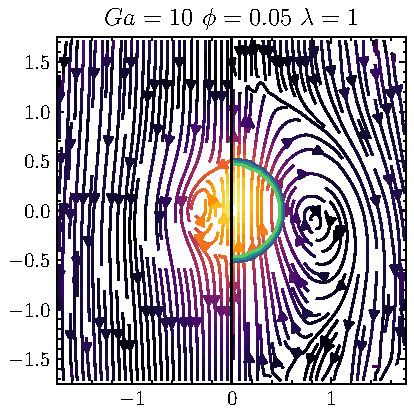
\includegraphics[height=0.25\textwidth]{image/HOMOGENEOUS/Stream/Stream_PHI_5_Ga_10_l_1.pdf}};
        \node (img) at (0.25\textwidth,0)  {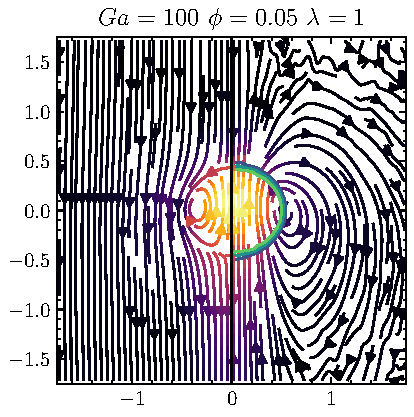
\includegraphics[height=0.25\textwidth]{image/HOMOGENEOUS/Stream/Stream_PHI_5_Ga_100_l_1.pdf}};
        \node (img) at (0.5\textwidth,0)  {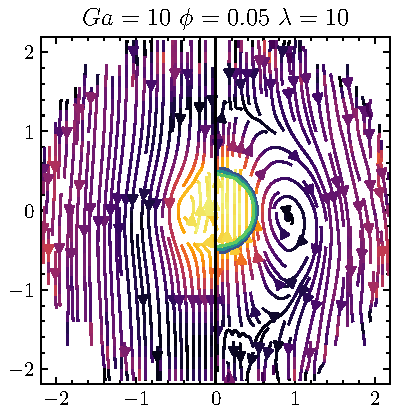
\includegraphics[height=0.25\textwidth]{image/HOMOGENEOUS/Stream/Stream_PHI_5_Ga_10_l_10.pdf}};
        \node (img) at (0.75\textwidth,0)  {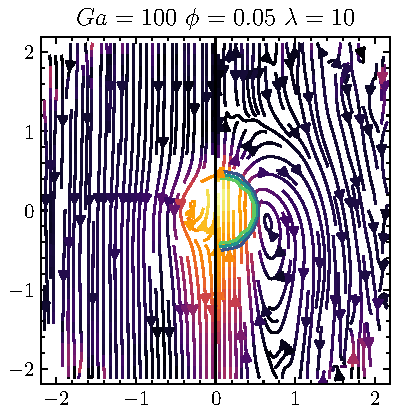
\includegraphics[height=0.25\textwidth]{image/HOMOGENEOUS/Stream/Stream_PHI_5_Ga_100_l_10.pdf}};
    \end{tikzpicture}
    \caption{Nearest particle averaged velocity $\nstavg{\textbf{u}}(\textbf{r})$ for  $\phi = 5\%$ and $20\%$.
    Green lines : contour plots of the nearest averaged indicator function $\nstavg{\chi_d}(\textbf{r})$ (it represent the mean shape of the particles)}
    \label{fig:Stream}
  \end{figure}
  
  \begin{itemize}
    \item Close from the drop ($r=\mathcal{O}(a)$) we can see that $\textbf{u}_\text{nst} \approx \textbf{u}_\text{stokes}$. 
  \end{itemize}
\end{frame}

\begin{frame}
  \frametitle{Nearest particle statistic solution for translating drops in stokes flow :}
  \begin{multline}
    \avg{\chi_f \textbf{u}'_f\textbf{u}'_f}(\textbf{x},t)
    = 
    {\int_a^\infty \textbf{u}_\text{stokes} \textbf{u}_\text{stokes}  P_{nst}(\textbf{x},t,\textbf{r}) d\textbf{r} }
    - \phi_f \textbf{u}_f\textbf{u}_f
    \\=
-\left({{-\left(9\,\Gamma\left(-1 , \,\phi\right)\,\lambda^2\,\phi
^{{{4}\over{3}}}\,e^{\phi}\right)+\ldots}\over{\left(120\,\lambda^2+240\,\lambda+
120\right)\,\phi^{{{1}\over{3}}}}}\right)
\textbf{e}_U\textbf{e}_U + \ldots
\end{multline}
\begin{itemize}
  \item $\textbf{e}_U$ is the units vector in the direction of the drift velocity. 
\end{itemize}

\end{frame}

\begin{frame}
  \frametitle{Comparison with DNS results and experiments}
  \begin{figure}[h!]
    \centering    
    % 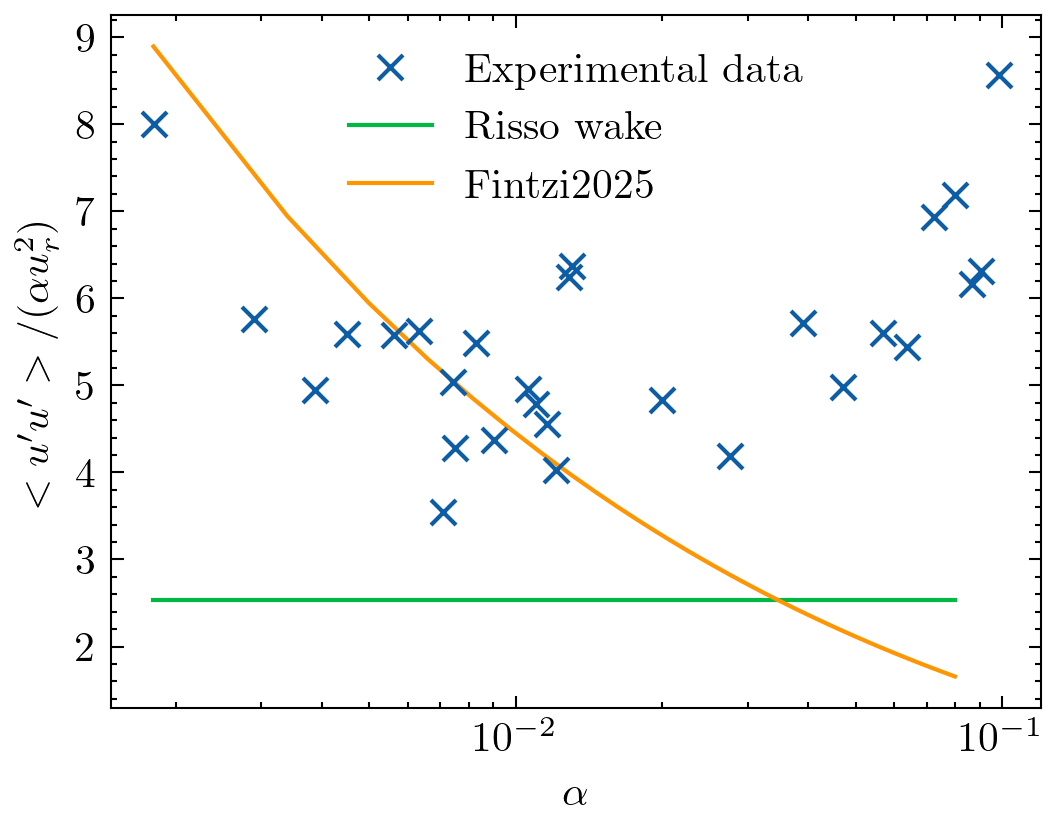
\includegraphics[height = 0.25\textwidth]{image/upupexp.png}
    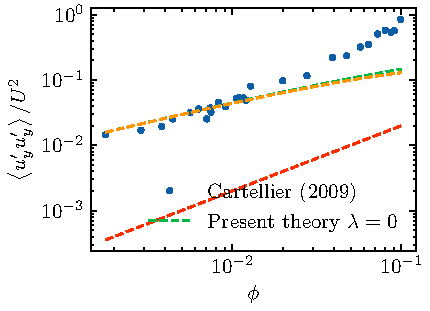
\includegraphics[height = 0.25\textwidth]{image/HOMOGENEOUS/fCA/cartellier.pdf}
    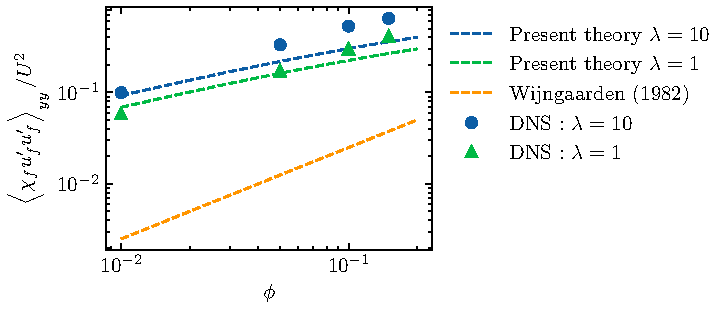
\includegraphics[height = 0.25\textwidth]{image/HOMOGENEOUS/fCA/Pseudo_turbe.pdf}
    \caption{
       Dimensionless \textbf{fluid phase pseudo kinetic energy} :
       (left) Comparison with the rising bubbles experiment of Cartellier (2009) with $Re \approx 10$. 
       (right) comparison with DNS for two viscosity ratio $\lambda =1,10$ and $Re \approx 1$ DNS. 
    }
    \label{fig:Cp}
\end{figure}  
\begin{itemize}
  \item The tendency in terms of $\phi$ and $\lambda$ are right.  
  \item Quantitative agreement at $\phi \ll 1$ and not at $\phi <1$ because of the interactions.  
  \item The present theory solution indeed diverge in $\phi \to 0$ 
\end{itemize}
\end{frame}

\begin{frame}
  \frametitle{Comparison with DNS results }
  \begin{figure}[h!]
    \centering    
    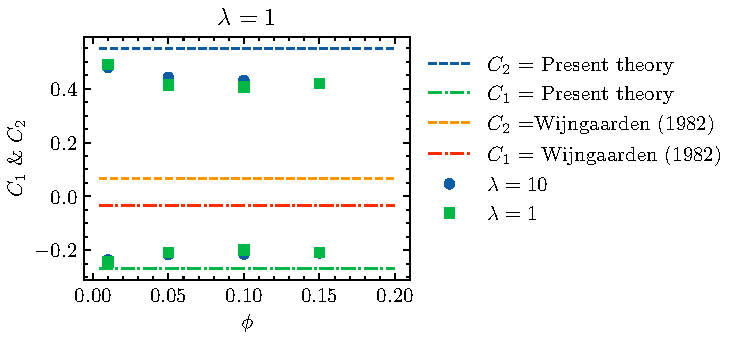
\includegraphics[height = 0.25\textwidth]{image/HOMOGENEOUS/fCA/Pseudo_turbe_coef.pdf}
    \caption{
       Coefficient of the Reynolds stress tensor in terms of the volume fraction $\phi$ for two viscosity ratio $\lambda =1,10$ and $Re \approx 1$ DNS. 
    }
    \label{fig:Cp}
\end{figure}  
Where we have defined :
\begin{equation*}
  \avg{\chi_1\textbf{u}_1'\textbf{u}_1'}
  = k^*_1 \left[
      \textbf{U}
      \textbf{U}
      (C_1  - C_2 )
      + \textbf{I} 
      (\textbf{U}\cdot\textbf{U})  (C_1+2/3) 
  \right]
\end{equation*}
\end{frame}


\begin{frame}
  \frametitle{Particle phase kinetic energy}
  Assuming \textbf{force free} particle in stokes flow one can also derive the Reynolds stress from nearest particle statistic. 
  \begin{figure}[h!]
    \centering    
    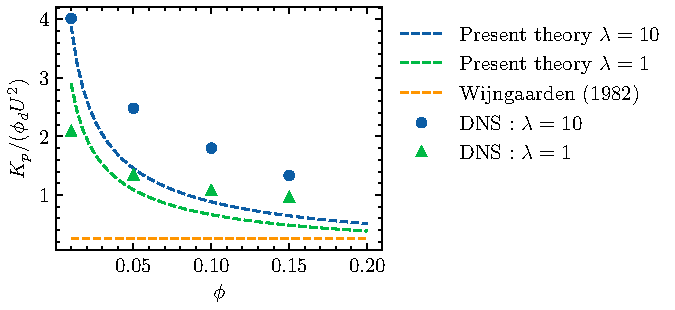
\includegraphics[height = 0.25\textwidth]{image/HOMOGENEOUS/fCA/Pseudo_turbeP.pdf}
    \caption{
       Dimensionless \textbf{granular temperature} in terms of the volume fraction $\phi$ for two viscosity ratio $\lambda =1,10$ and $Re \approx 1$ DNS. 
    }
    \label{fig:Cp}
\end{figure}  
\begin{itemize}
  \item The tendency in terms of $\phi$ and $\lambda$ are right.  
  \item Quantitative agreement at $\phi \ll 1$.  
\end{itemize}


\end{frame}
\begin{frame}
  {Perspectives}
  \begin{itemize}
    \item Takes in account interactions between particle with reflexion method 
    \item Takes in account inertial effect Using Ossen wake. 
    \item Can also compute : $\avg{\chi_1 \bm{\sigma}_1^0 : \grad  \textbf{u}_0^1}$ and other closure terms. 
  \end{itemize}
\end{frame}
\end{document}
